\subsection{Background}
Virtual Reality (VR) technology is an area of wearables that have been on the rise
as computer hardware capabilities improve. The Virtual Reality Society defines VR as
a 3D environment generated by a computer that a person can interact with, and be
immersed in such a way that the person can manipulate and interact with the environment
much like they would in \textit{actual} reality \cite{vr_soc_defn}. High-quality
technology and intelligent architectures are required to realize VR due to
the compute-intensive task of processing many inputs and rendering a virtual
world/environment in real time, and depending on the level of detail (LoD), is
an intensive task on its own \cite{hickey_wt4_pres}. Therefore, it is necessary
to make intelligent architecture design decisions to ensure the VR wearable operates
as intended, and with the correct performance specifications.

The most common type of VR wearable is the VR headset, and example is shown below in
Figure \ref{vr:example}. As illustrated, the headset is worn on the head (making it
a wearable), and its screen takes up the user's entire field of view - thereby immersing
them in a virtual environment. Some headsets include audio capabilities and movement
sensors, but this will be discussed later in this section.


\begin{figure}[h]
    \centering
    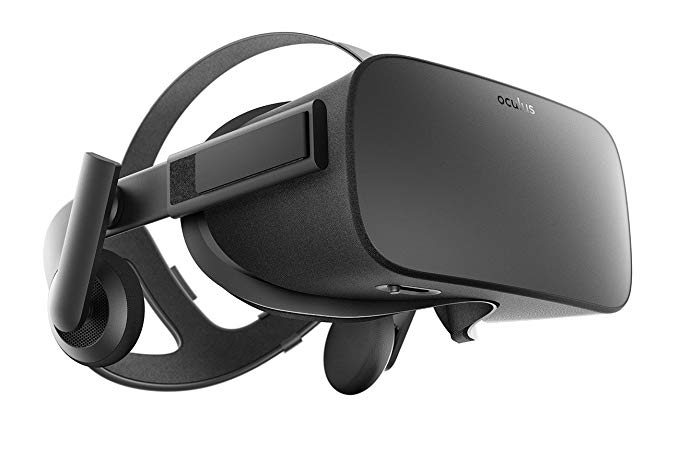
\includegraphics[width=.3\linewidth]{media/vr_headset_example.jpg}
    \caption{Apple S5 Processor \cite{vr_headset_pic}}
    \label{vr:example}
\end{figure}

\subsection{Typical Use Cases}
Due to the immersive and potentially high-fidelity rendering that VR can accomplish,
there are several key applications where this technology can be applied. For example, 
VR has the potential for entertainment, business, and medical applications.

For entertainment applications, VR has the potential to revolutionize video games.
Keep writing...

For business applications, VR can be used for modelling buildings before they break
ground, but also for completing expensive and dangerous training exercises at a lower
cost, and with zero risk - like ExxonMobil has started doing recently \cite{exxon_vr}.